\providecommand{\main}{../../..}
\documentclass[\main/main.tex]{subfiles}
\begin{document}

\subsection{Esercizio 2}
Dato il problema di programmazione matematica

\begin{align*}
  \min f(x) & = (x_1+1)^2 + (x_2 + \frac{1}{2})^2 \\
  g_1(x)    & = x_1 - x_2 \leq 0                  \\
  g_2(x)    & = x_1 + x_2 \geq 0                  \\
  g_3(x)    & = x_3 \geq 0                        \\
\end{align*}

\begin{enumerate}[a)]
  \item Si rappresenti il problema graficamente.
  \item Si determinino gli eventuali punti non regolari.
  \item Si determinino i punti candidati secondo le condizioni di KKT, e in particolare quello/i di minimo.
\end{enumerate}

\subsection{Soluzione esercizio 2}

\paragraph*{Riscrivo i vincoli}
\begin{align*}
  \min f(x) & = (x_1+1)^2 + (x_2 + \frac{1}{2})^2 \\
  g_1(x)    & = x_1 - x_2 \leq 0                  \\
  g_2(x)    & = -x_1 - x_2 \leq 0                 \\
  g_3(x)    & = -x_2 \leq 0                       \\
\end{align*}

\paragraph*{Rappresentazione grafica del problema}

\begin{figure}
  \begin{subfigure}{0.45\textwidth}
    \begin{tikzpicture}
      \begin{axis}[
          grid=major,
          samples=\samples,
          xlabel=$x_1$,
          ylabel=$x_2$,
          zlabel=$f(x)$
        ]
        \addplot3[surf, unbounded coords=jump]
        {x - y < 0 && -x -y <0 && y > 0 ? (x+1)^2 + (y + 0.5)^2 : NaN};
      \end{axis}
    \end{tikzpicture}
    \caption{La funzione $f(x)$}
    \label{func}
  \end{subfigure}
  ~
  \begin{subfigure}{0.45\textwidth}
    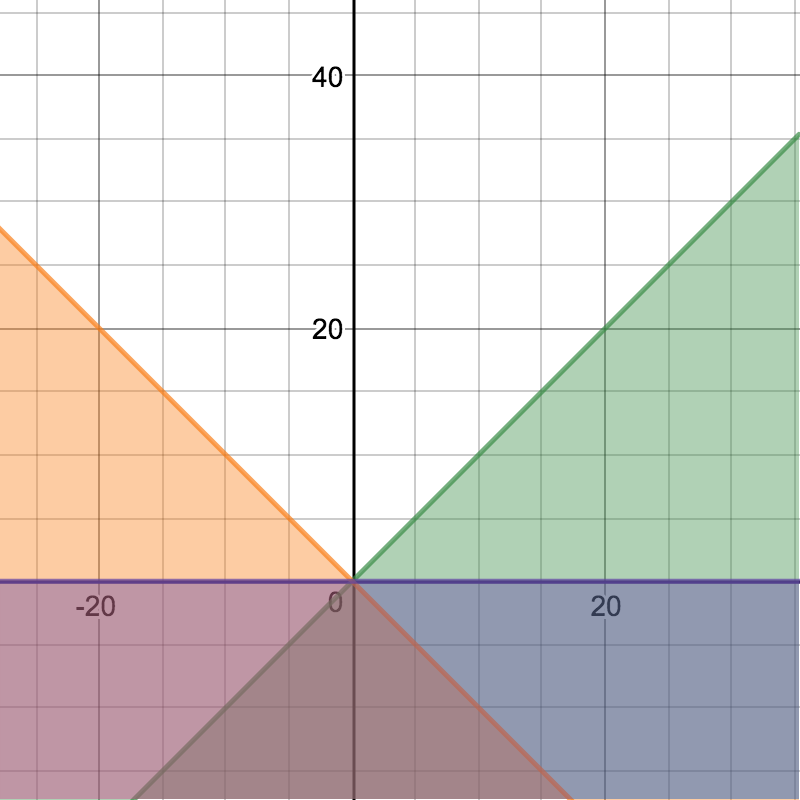
\includegraphics[width=0.8\textwidth]{20160322domain}
    \caption{Dominio della funzione $f(x)$}
  \end{subfigure}
\end{figure}

\paragraph*{Calcolo dei punti non regolari}

\subparagraph*{Calcolo i gradienti dei vincoli}

\[
  \nabla g_1 = \begin{bmatrix}
    1 \\
    -1
  \end{bmatrix}
  \qquad
  \nabla g_2 = \begin{bmatrix}
    -1 \\
    -1
  \end{bmatrix}
  \qquad
  \nabla g_3 = \begin{bmatrix}
    0 \\
    -1
  \end{bmatrix}
\]

Nessuno dei gradienti si può annullare.

\subparagraph*{Calcolo dei punti di intersezione dei vincoli}
L'unico punto di intersezione esistente è l'origine $O=(0,0)$. Questo punto è regolare poichè non rende singolare la matrice dei gradienti (che non può mai annullarsi).

\paragraph*{Condizioni di KKT}

\subparagraph*{Costruisco la lagrangiana generalizzata}

\[
  l(x) = (x_1+1)^2 + (x_2 + \frac{1}{2})^2 + \mu_1(x_1 - x_2) - \mu_2(x_1 + x_2) - \mu_3x_2
\]

\subparagraph*{Costruisco il sistema delle condizioni KKT}
\[
  \begin{cases}
    \nabla l(x) = \begin{bmatrix}
      2(x_1+1) + \mu_1 - \mu_2                   \\
      2(x_2+\frac{1}{2}) - \mu_1 - \mu_2 - \mu_3 \\
    \end{bmatrix} = \bm{0} \\
    \mu_1(x_1 - x_2) = 0                             \\
    \mu_2(x_1 + x_2) = 0                             \\
    \mu_3x_2 = 0                                     \\
    x_1 - x_2 \leq 0                                 \\
    x_1 + x_2 \geq 0                                 \\
    x_2 \geq 0                                       \\
    \mu_1 \geq 0                                     \\
    \mu_2 \geq 0                                     \\
    \mu_3 \geq 0                                     \\
  \end{cases}
\]

Porre a $0$ uno qualsiasi dei vincoli significa imporre pari a $0$ tutti i vincoli, dato che l'origine è un punto di intersezione dei tre vincoli.

\subparagraph*{Caso $\mu_3 = 0 \land g_3 < 0$:}

\[
  \begin{cases}
    \nabla l(x) = \begin{bmatrix}
      2(x_1+1) + \mu_1 - \mu_2           \\
      2(x_2+\frac{1}{2}) - \mu_1 - \mu_2 \\
    \end{bmatrix} = \bm{0} \\
    \mu_1(x_1 - x_2) = 0                              \\
    \mu_2(x_1 + x_2) = 0                              \\
    x_1 - x_2 \leq 0                                  \\
    x_1 + x_2 \geq 0                                  \\
    x_2 > 0                                           \\
    \mu_1 \geq 0                                      \\
    \mu_2 \geq 0                                      \\
    \mu_3 = 0                                         \\
  \end{cases}
\]

Spezzo il problema in due ulteriori sotto casi: $P_1: g_2<0 \land \mu_2=0$

\[
  \begin{cases}
    \nabla l(x) = \begin{bmatrix}
      2(x_1+1) + \mu_1           \\
      2(x_2+\frac{1}{2}) - \mu_1 \\
    \end{bmatrix} = \bm{0} \\
    \mu_1(x_1 - x_2) = 0                              \\
    x_1 - x_2 \leq 0                                  \\
    x_1 > -x_2                                        \\
    x_2 > 0                                           \\
    \mu_1 \geq 0                                      \\
    \mu_2 = 0                                         \\
    \mu_3 = 0                                         \\
  \end{cases}
  \Rightarrow
  \begin{cases}
    \error{x_1+1 + x_2+\frac{1}{2} = 0 \Rightarrow x_1 = -\frac{3}{2} - x_2} \\
    \mu_1(x_1 - x_2) = 0                                                     \\
    x_1 - x_2 \leq 0                                                         \\
    \error{x_1 > -x_2}                                                       \\
    x_2 > 0                                                                  \\
    \mu_1 \geq 0                                                             \\
    \mu_2 = 0                                                                \\
    \mu_3 = 0                                                                \\
  \end{cases}
\]

Il sistema risulta impossibile.

L'unico punto che risolve il sistema delle condizioni KKT rimane quindi l'origine.

\paragraph*{Calcolo del valore del punto ottimo}
L'unico punto candidato che rimane è $O = (0,0)$
\[
  f(O) = f(0,0) = 1.25
\]

\end{document}